\documentclass[12pt]{article}
\usepackage[margin=1in]{geometry}
\usepackage{amsmath}
\usepackage{amssymb}
\usepackage{amsthm}
\usepackage{matlab-prettifier}
\usepackage{graphicx}
\usepackage{hyperref}
\usepackage{pgfplots}
\usepackage{tikz}
\usepackage{tikz-3dplot}
\usepackage{pgfplots}
\usetikzlibrary{arrows.meta}
\usepackage{fancyhdr}
\usepackage{multirow, multicol}
\usepackage{enumitem}
\usepackage{caption}
\usepackage{subcaption}
\usepackage{tabu}
\pagestyle{fancy}
\hypersetup{
  colorlinks=true,
  linkcolor=blue,
  filecolor=magenta,      
  urlcolor=cyan,
}

\theoremstyle{definition}
\newtheorem*{notation}{Notation}
\newtheorem*{definition}{Definition}
\usepackage{comment}
\newenvironment{solution}{
 \par\noindent\ignorespaces\textbf{Solution.}}{\newpage}
\renewcommand*{\thefootnote}{\fnsymbol{footnote}\fnsymbol{footnote}}
%% -----------------

\parindent 0pt
\parskip 10pt

\fancyhead[RO]{MATH-GA2020}
\fancyhead[LO]{Final Project due Monday May 12 2025}

\begin{document}

\begin{center}
{\Large MATH-GA 2020 Numerical Methods II\\ Numerical Simulation of the Stefan Problem}

\end{center}

\section{Background}
Many natural and industrial processes—melting of ice, solidification of metals, thawing of permafrost—involve a moving interface separating distinct phases. Mathematically, these are free-boundary problems, since the location of the phase interface is part of the unknown. The prototypical model is called the Stefan problem, named after Josef Stefan, who in the late 19th century analyzed heat diffusion in ice formation on polar seas. In its classical form, we seek both the temperature $u(x,t)$ and the moving interface $\Gamma(t)$, which separates the solid and liquid phases. 

In this project, only the one phase Stefan problem is considered, where one of the two phases (typically the solid) remains at the constant melting temperature $T_m$, so that only the temperature in the other phase should be solved. 

\section{One Dimensional Stefan Problem}
\subsection{Mathematical Formulation}
Consider a semi-infinite one-dimensional block of ice initially at melting temperature $u(x,0) = T_m$ for $x \in (0, \infty)$, a constant temperature $T_l > T_m$ is imposed at the left boundary $x=0$ for $t > 0$, and the ice is allowed to melt into water and left a region of water $[0, \Gamma(t))$ at time $t$. Here, $\Gamma(t)$ is the position of the melting front at time $t$. The problem is governed by the following equations:
\begin{equation}
\begin{aligned}
  &u_t = \alpha u_{xx}, \quad x \in [0, \Gamma(t)), t > 0, \\
  &u(0,t) = T_l, \quad u(\Gamma(t),t) = T_m \quad t > 0, \\
  &\beta \frac{d}{dt} \Gamma(t) = -\alpha u_x(\Gamma(t),t), \quad t > 0, \\
  &u(x,0) = T_m, \quad x \in [0, \infty), \\
  &\Gamma(0) = \gamma_0
\end{aligned}
\end{equation}
where $u_t$ and $u_{xx}$ are the first and second spatial derivatives of $u$, respectively, $\alpha$ is the thermal diffusivity, $\beta$ is the Stefan number, the ratio of latent to specific sensible heat. The first equation is the heat equation, which describes the temperature distribution in the solid phase. The second equation is the boundary condition at the left boundary and the melting front. The third equation is the Stefan condition. The fourth and fifth equation are the initial conditions of temperature and the melting front.

For one dimensional one phase Stefan problem, we can find an analytical solution which is called the Neumann solution. It's obtained by using self-similar variables. The solution is given by:
\begin{equation}
  \begin{aligned}
    &\Gamma(t) = 2 \lambda \sqrt{\alpha t}, \quad \text{where } \beta \lambda = \frac{1}{\sqrt{\pi}} \frac{e^{-\lambda^2}}{\text{erf}(\lambda)} \\
    &u(x,t) = T_l + (T_m - T_l) \frac{\text{erf}(\eta)}{\text{erf}(\lambda)},
    \quad \text{where } \eta = \frac{x}{2\sqrt{\alpha t}}
  \end{aligned}
\end{equation}
With such analytical solution, we can use it to verify the numerical methods.

\subsection{Front Tracking Method}
The first numerical method to solve this problem is front tracking method. The key idea of this method is tracking the moving interface $\Gamma(t)$ at each time step. We a fixed Eulerian grid (by finite difference) to solve the heat equation in the liquid region, that is $x_j = j \Delta x$ for $j = 0, 1, \ldots, N$, where $\Delta x$ is the grid size and $N$ is the number of grid points. Also, we have the time grid $t^n = n \Delta t$. For each time step $n$, the interface point $\Gamma^n$ is located between two grid points $x_{k(n)}$ and $x_{k(n)+1}$, where $k(n)$ is the index depending on time step $n$. 

Then at each time step from $n$ to $n+1$, we can use the following algorithm to update the temperature and the interface position:
\begin{enumerate}
  \item Update the temperature $u_t = \alpha u_{xx}$ in the liquid region $0\leq x \leq \Gamma^n$ using backward Euler method. The backward Euler method is an implicit method, which is unconditionally stable. The finite difference scheme for the heat equation is given by:
  \begin{equation*}
    u_j^{n+1} = u_j^n + \alpha \frac{\Delta t}{\Delta x^2} (u_{j+1}^n - 2u_j^n + u_{j-1}^n), \quad j = 1, \ldots, k(n)-1
  \end{equation*}
  \item Compute the gradient at the front $\Gamma^n$, since $\Gamma^n$ is between $x_{k(n)}$ and $x_{k(n)+1}$, we can interpolate the gradient by
  \begin{equation*}
    \frac{\partial u}{\partial x} \approx \frac{u_{k(n)+1}^n - u_{k(n)}^n}{\Delta x}
  \end{equation*}
  \item Update the interface position $\Gamma^{n+1}$ using the Stefan condition:
  \begin{equation*}
    \beta \frac{\Gamma^{n+1} - \Gamma^{n}}{\Delta t} = -\alpha \frac{u_{k(n)+1}^n - u_{k(n)}^n}{\Delta x}
  \end{equation*}
  \item Update the index $k(n+1)$ to make sure position $\Gamma^{n+1}$ is between $x_{k(n+1)}$ and $x_{k(n+1)+1}$.
  \item Optionally we can re-interpolate $u^{n}$ onto the grid point $j = 0, \ldots, k(n+1)$ and setting $T_{k(n+1)}^{n+1} = T_m$.
  \item Repeat until finish.
\end{enumerate}

\begin{figure*}[h!]
  \centering
  \begin{subfigure}[b]{0.47\textwidth}
    \centering
    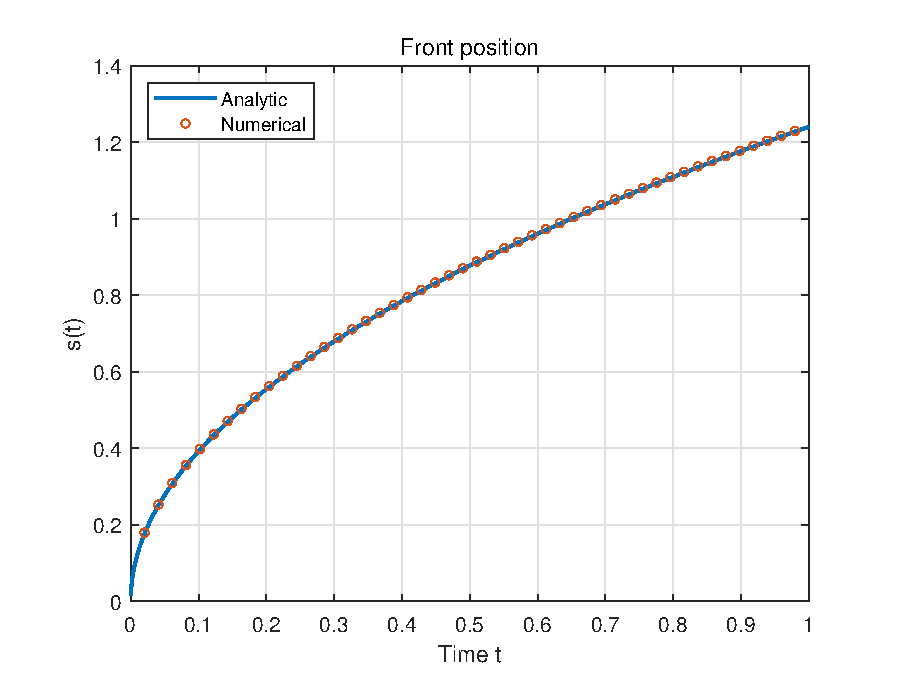
\includegraphics[width=\textwidth]{./figures/figure_1.eps}
    \label{fig:1a}
  \end{subfigure}
  \begin{subfigure}[b]{0.47\textwidth}
    \centering
    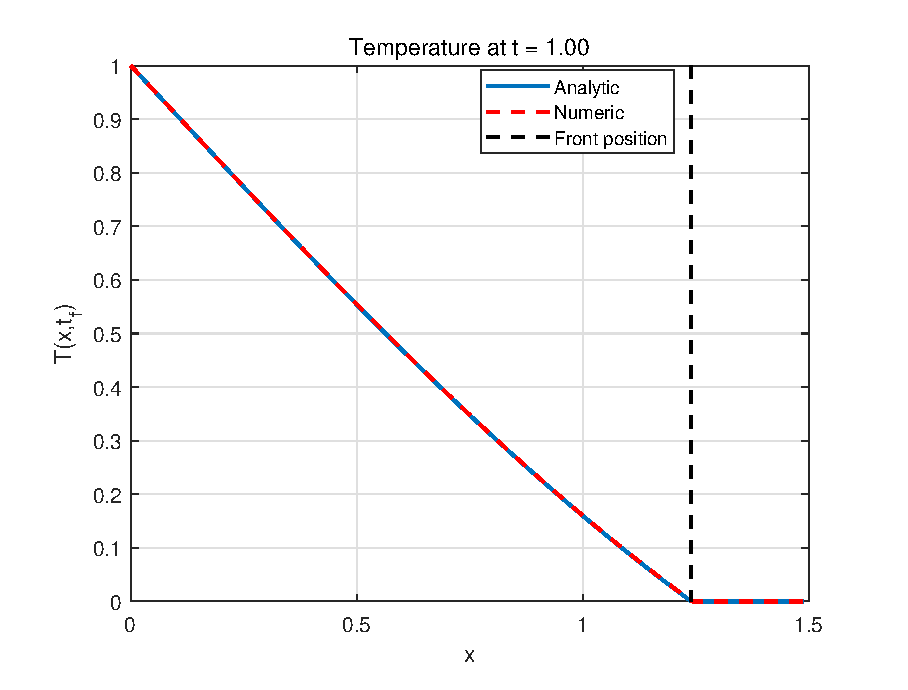
\includegraphics[width=\textwidth]{./figures/figure_2.eps}
    \label{fig:1b}
  \end{subfigure}
  \caption{The interface position $\Gamma(t)$ and the temperature $u(x,t)$ at final time $t=1$}
  \label{fig:1}
\end{figure*}

From the figures \ref{fig:1}, we can see for one dimensional Stefan problem, the results computed by the front tracking method are matched well for the analytical solution. The interface position $\Gamma(t)$ looks like a square root function of time, and the temperature $u(x,t)$ is quasi-linear function of $x$. 

The front tracking method is a simple and efficient method to solve the free boundary problem. However, it has some limitations with the convergence order. The convergence order of the front tracking method is only first order. 
\begin{figure*}[h!]
  \centering
  \begin{subfigure}[b]{0.47\textwidth}
    \centering
    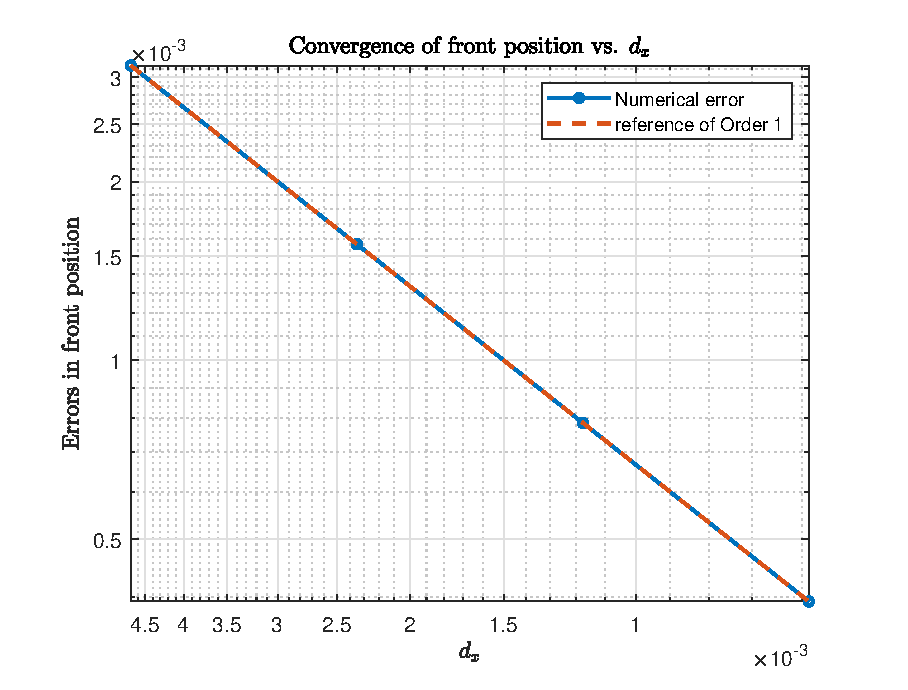
\includegraphics[width=\textwidth]{./figures/figure_3.eps}
    \label{fig:3a}
  \end{subfigure}
  \begin{subfigure}[b]{0.47\textwidth}
    \centering
    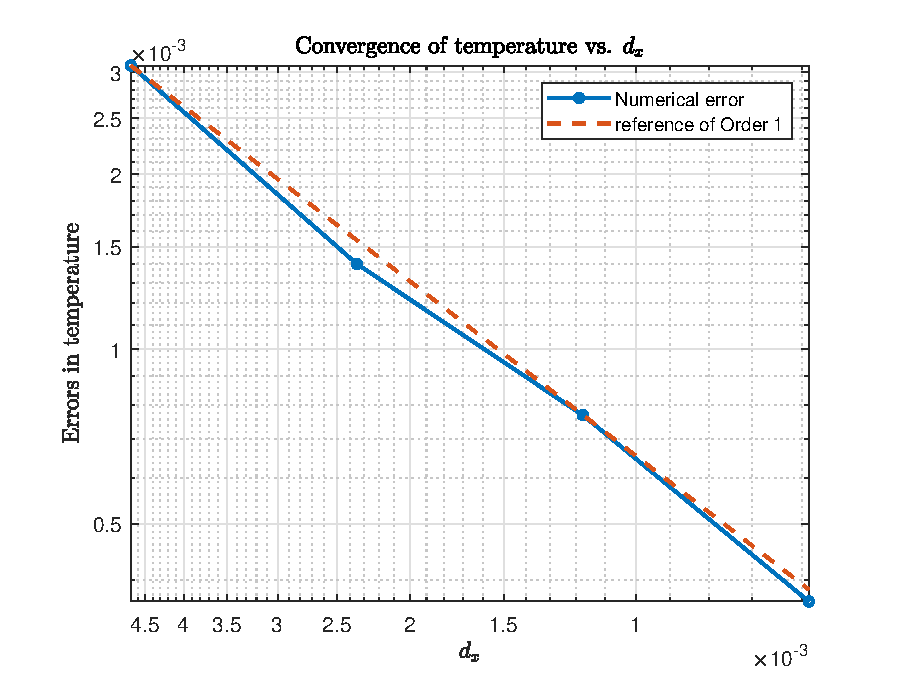
\includegraphics[width=\textwidth]{./figures/figure_4.eps}
    \label{fig:3b}
  \end{subfigure}
  \caption{The convergence order of front position and temperature with respect to $d_x$}
  \label{fig:3}
\end{figure*}

The convergence order of the front position $\Gamma(t)$ and the temperature $u(x,t)$ with respect to the grid size $\Delta x$ is shown in figure \ref{fig:3}. The convergence order is about 1.0. This is due to the update equation $\beta \frac{\Gamma^{n+1} - \Gamma^{n}}{\Delta t} = -\alpha \frac{u_{k(n)+1}^n - u_{k(n)}^n}{\Delta x}$ is only first order. 

\begin{figure*}[h!]
  \centering
  \begin{subfigure}[b]{0.47\textwidth}
    \centering
    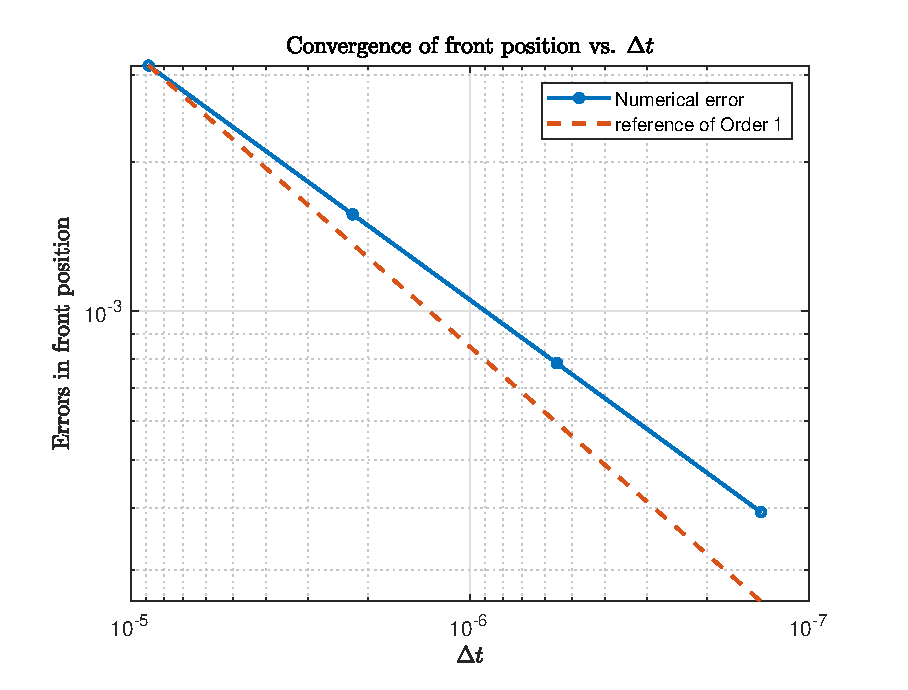
\includegraphics[width=\textwidth]{./figures/figure_5.eps}
    \label{fig:5a}
  \end{subfigure}
  \begin{subfigure}[b]{0.47\textwidth}
    \centering
    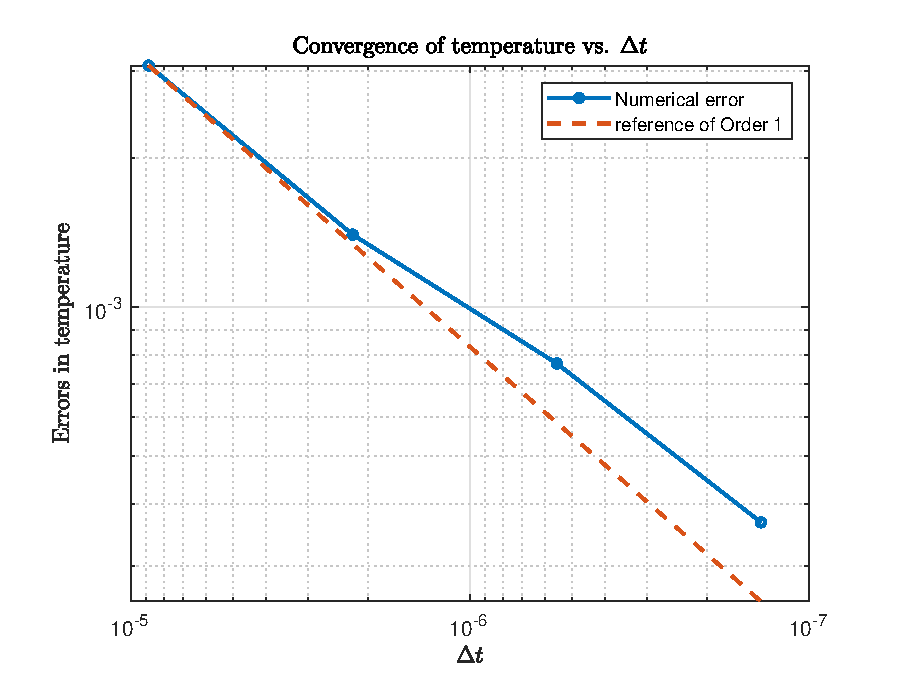
\includegraphics[width=\textwidth]{./figures/figure_6.eps}
    \label{fig:5b}
  \end{subfigure}
  \caption{The convergence order of front position and temperature with respect to $d_t$}
  \label{fig:5}
\end{figure*}

The convergence order of the front position $\Gamma(t)$ and the temperature $u(x,t)$ with respect to the time step $\Delta t$ is shown in figure \ref{fig:5}. The convergence order is little bit less 1.0. I think the main factor is that we need to use two first order methods to update the front position $\Gamma(t)$. Thus, it reduces the convergence order.

\subsection{Level Set Method}
The second numerical method to solve this problem is level set method. The key idea of this method is to use a level set function $\phi(x,t)$ to represent the interface position $\Gamma(t)$. The level set function is a signed distance function, which is positive in the liquid region and negative in the solid region. The interface position is given by the zero level set of the level set function, that is $\Gamma(t) = \{x | \phi(x,t) = 0\}$. 

Initially we can set the level set function as:
\begin{equation*}
  \phi(x,0) = \begin{cases}
    x - \gamma_0, & x < \gamma_0 \\
    0, & x = \gamma_0 \\
    x - \gamma_0, & x > \gamma_0
  \end{cases}
\end{equation*}
where $\gamma_0$ is the initial position of the interface. Then its evolution is governed by the Hamilton-Jacobi equation:
\begin{equation*}
  \frac{\partial \phi}{\partial t} + V \cdot |\nabla \phi| = 0, \quad x \in [0, \infty), t > 0
\end{equation*}
Here in one dimensional case, we can reduces the Hamilton-Jacobi equation to:
\begin{equation*}
  -\frac{\partial}{\partial t} \Gamma(t) + V = 0 \Rightarrow V = \frac{\partial }{\partial t}\Gamma(t)
\end{equation*}

Then at each time step, we do 
\begin{enumerate}
  \item We regard the region which $\phi(x,t) < 0$ as the liquid region and $\phi(x,t) > 0$ as the solid region.
  \item Solve the heat equation in the liquid region $\phi(x,t) < 0$ using the finite difference method. The finite difference scheme for the heat equation is given by:
  \begin{equation*}
    u_j^{n+1} = u_j^n + \alpha \frac{\Delta t}{\Delta x^2} (u_{j+1}^n - 2u_j^n + u_{j-1}^n), \quad j = 1, \ldots, N
  \end{equation*}
  \item Compute the update of the level set function $\phi(x,t)$ using the Hamilton-Jacobi equation, $V$ is according to the Stefan condition.
  \item Update the level set function $\phi(x,t)$, and the new interface position $\Gamma(t)$ is given by the zero level set of the level set function, that is $\Gamma(t) = \{x | \phi(x,t) = 0\}$.
  \item For several time steps, we can re-initialize the level set function to make sure it is a signed distance function. The re-initialization can be done by solving the following equation:
  \begin{equation*}
    \phi_t = sign(\phi_0) \left(1 - |\nabla \phi|\right)
  \end{equation*}
\end{enumerate}

The major difference between the level set method and the front tracking method is that the level set method does not need to track the interface position explicitly. This makes the level set method easier to generalize to higher dimensions and more complex geometries.
\begin{figure*}[h!]
  \centering
  \begin{subfigure}[b]{0.47\textwidth}
    \centering
    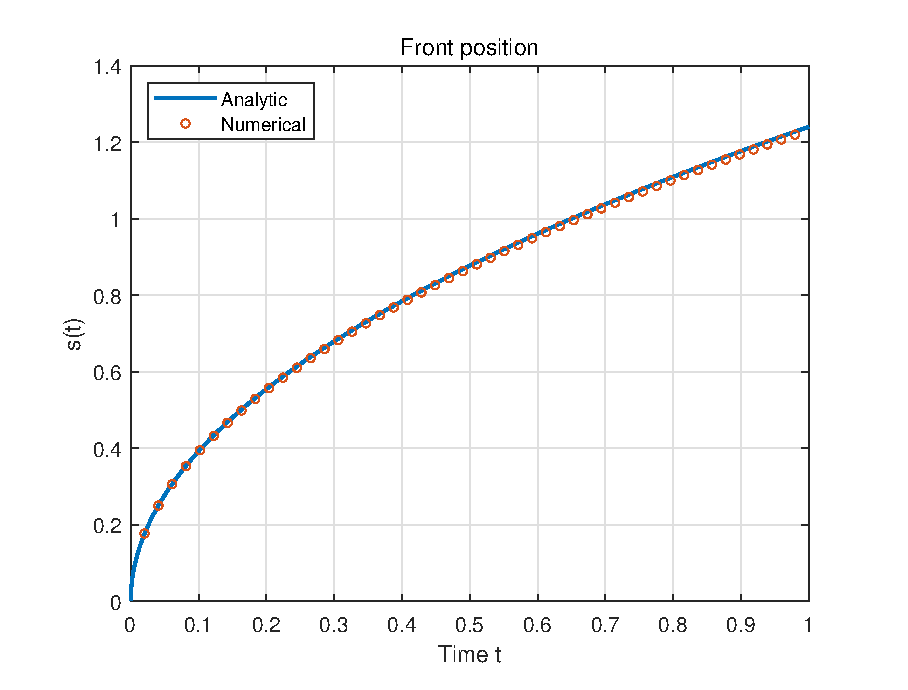
\includegraphics[width=\textwidth]{./figures/figure_7.eps}
    \label{fig:7a}
  \end{subfigure}
  \begin{subfigure}[b]{0.47\textwidth}
    \centering
    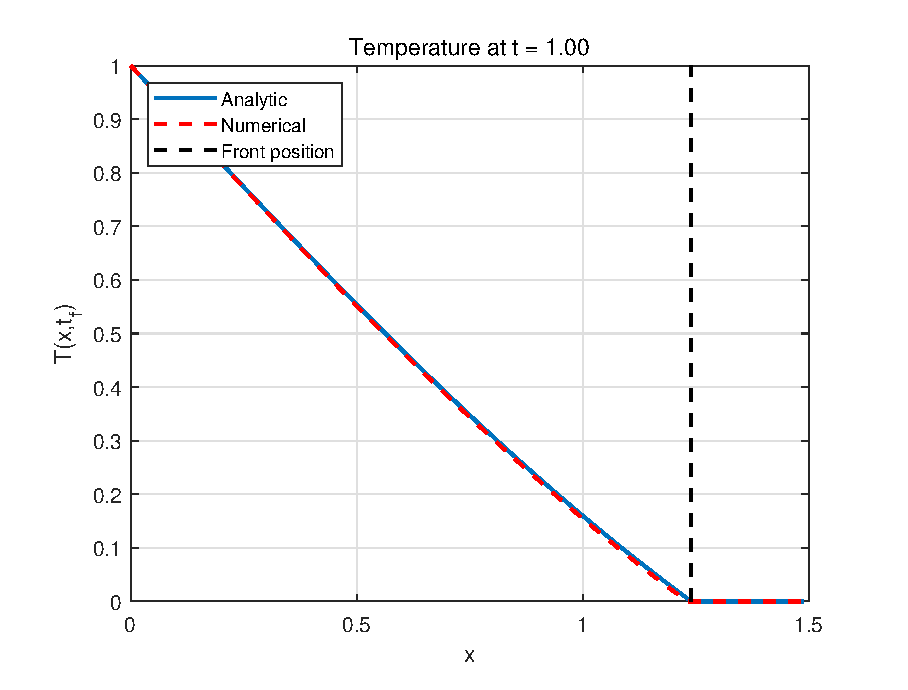
\includegraphics[width=\textwidth]{./figures/figure_8.eps}
    \label{fig:7b}
  \end{subfigure}
  \caption{The temperature profile and final interface position at $t=1$}
  \label{fig:7}
\end{figure*}

As figure \ref{fig:7} show, the results computed by the level set method also yield a good approximation to the analytical solution. The convergence order of front position $\Gamma(t)$ is similar to the front tracking method. But for the temperature $u(x,t)$, the level set method convergence slower than the front tracking method. This is because the re-initialization process will introduce some numerical errors, which will affect the convergence order of the temperature. The accuracy will be affected by the frequency of re-initialization, if the time step is small, we don't need to re-initialize the level set function frequently, and if we don't re-initialize the level set function at all, for the one dimensional case, the level set method will deduce to the front tracking method except it handles all the grid points in both solid and liquid regions.

\begin{figure*}[h!]
  \centering
  \begin{subfigure}[b]{0.47\textwidth}
    \centering
    \includegraphics[width=\textwidth]{./figures/figure_9.eps}
    \label{fig:9a}
  \end{subfigure}
  \begin{subfigure}[b]{0.47\textwidth}
    \centering
    \includegraphics[width=\textwidth]{./figures/figure_10.eps}
    \label{fig:9b}
  \end{subfigure}
  \caption{The convergence order of front position and temperature with respect to $d_x$}
  \label{fig:9}
\end{figure*}

\begin{figure*}[h!]
  \centering
  \begin{subfigure}[b]{0.47\textwidth}
    \centering
    \includegraphics[width=\textwidth]{./figures/figure_11.eps}
    \label{fig:11a}
  \end{subfigure}
  \begin{subfigure}[b]{0.47\textwidth}
    \centering
    \includegraphics[width=\textwidth]{./figures/figure_12.eps}
    \label{fig:11b}
  \end{subfigure}
  \caption{The convergence order of front position and temperature with respect to $d_t$}
  \label{fig:11}
\end{figure*}

\section{Two Dimensional Stefan Problem}
\subsection{Mathematical Formulation}
For two dimensional Stefan problem, the major difference is that the interface position $\Gamma(t)$ is a curve in the two dimensional space. Now we have $\Omega(t) \subset \mathbb{R}^2$ that denotes the liquid region at time $t$, and the heat equation changes to:
\begin{equation*}
  u_t = \alpha \Delta u, \quad x \in \Omega(t), t > 0
\end{equation*}
where $\Delta u$ is the Laplace operator. The Stefan condition at $\Gamma(t)$ is also changed to:
\begin{equation*}
  \beta \frac{d}{dt} \Gamma(t) = -\alpha \frac{\partial u}{\partial n}, \quad t > 0
\end{equation*}
where $\frac{\partial u}{\partial n}$ is the normal derivative of $u$ at the interface $\Gamma(t)$. The boundary conditions are still the same as the one dimensional case. The initial conditions are also the same as the one dimensional case. The main difference is that we need to solve the heat equation in the liquid region $\Omega(t)$, which is a moving domain.

\subsection{Front Tracking Method}
For two dimensional Stefan problem, the scheme of front tracking method is similar to the one dimensional case. The main difference is that we need to track the interface position $\Gamma(t)$ in the two dimensional space and solve the Laplacian. The algorithm for two dimensional case is verified by set the initial condition as a vertical line at the left boundary, thus it just simply extend the one dimensional case to two dimensional case, then we can check the final position of the interface by the analytical solution. 
\begin{figure*}[h!]
  \centering
  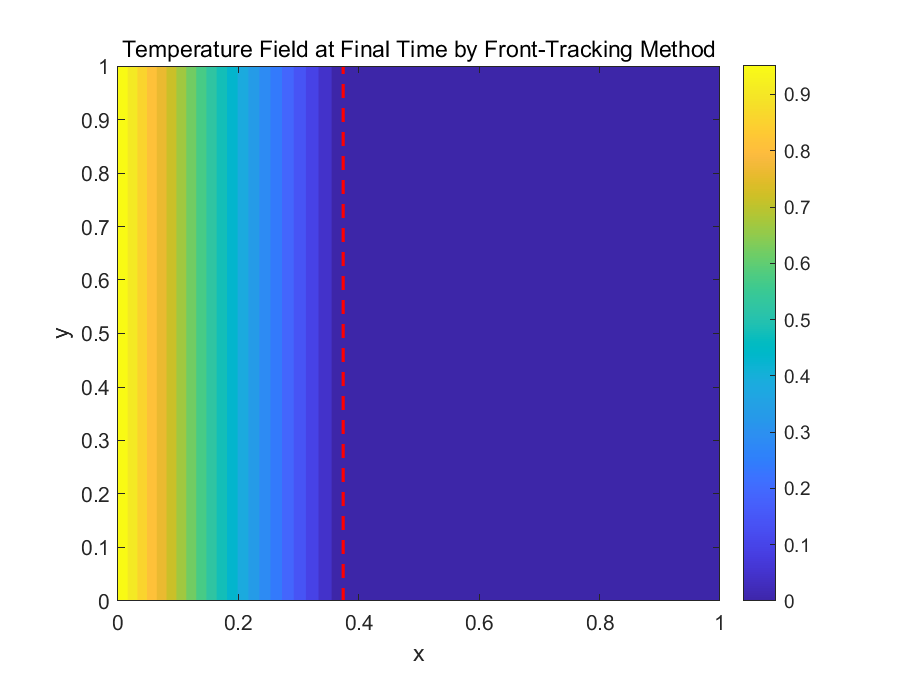
\includegraphics[width=0.5\textwidth]{./figures/figure_13.eps}
  \caption{The temperature profile and final interface position at $t=0.1$}
  \label{fig:13}
\end{figure*}
\begin{lstlisting}[style=Matlab-editor]
  With grid number 200, the error of interface position at final time is 1.799094e-02
\end{lstlisting}

\newpage
Then for a more complex case, the initial condition becomes a cirve $x = 0.5 + 0.1\sin(2\pi y)$, I use another method which is easy to implement (Enthalpy Method) to verify the result. The following figure shows the temperature profile and the final interface position at $t=0.1$.
\begin{figure}[h!]
  \centering
  \begin{subfigure}[b]{0.47\textwidth}
    \centering
    \includegraphics[width=\textwidth]{./figures/figure_14.eps}
    \label{fig:14a}
  \end{subfigure}
  \begin{subfigure}[b]{0.47\textwidth}
    \centering
    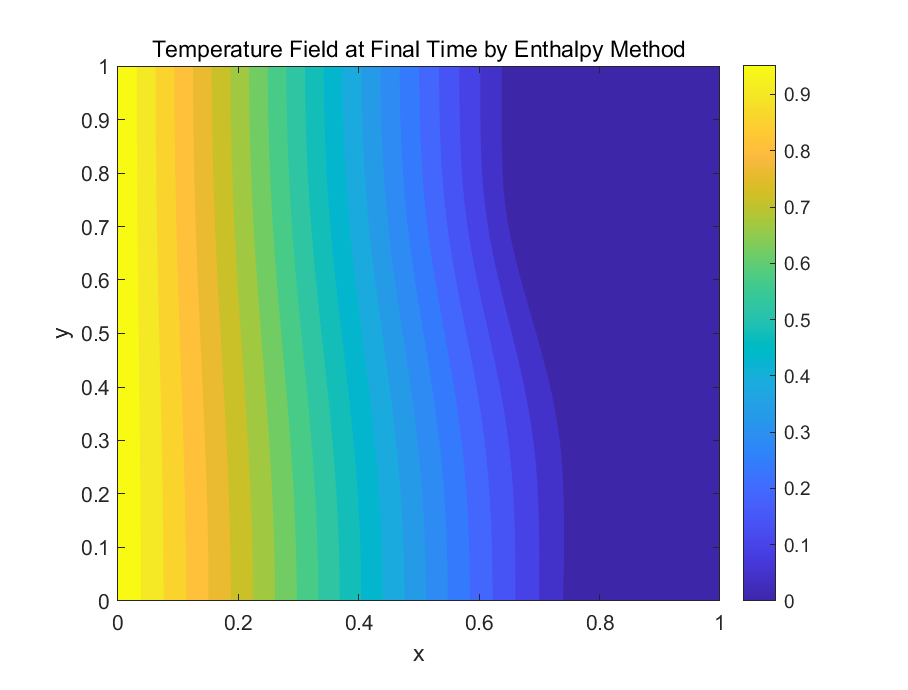
\includegraphics[width=\textwidth]{./figures/figure_15.eps}
    \label{fig:14b}
  \end{subfigure}
  \caption{The result for validation simulated by Enthalpy Method.}
  \label{fig:14}
\end{figure}

\begin{figure}[h!]
  \centering
  \begin{subfigure}[b]{0.47\textwidth}
    \centering
    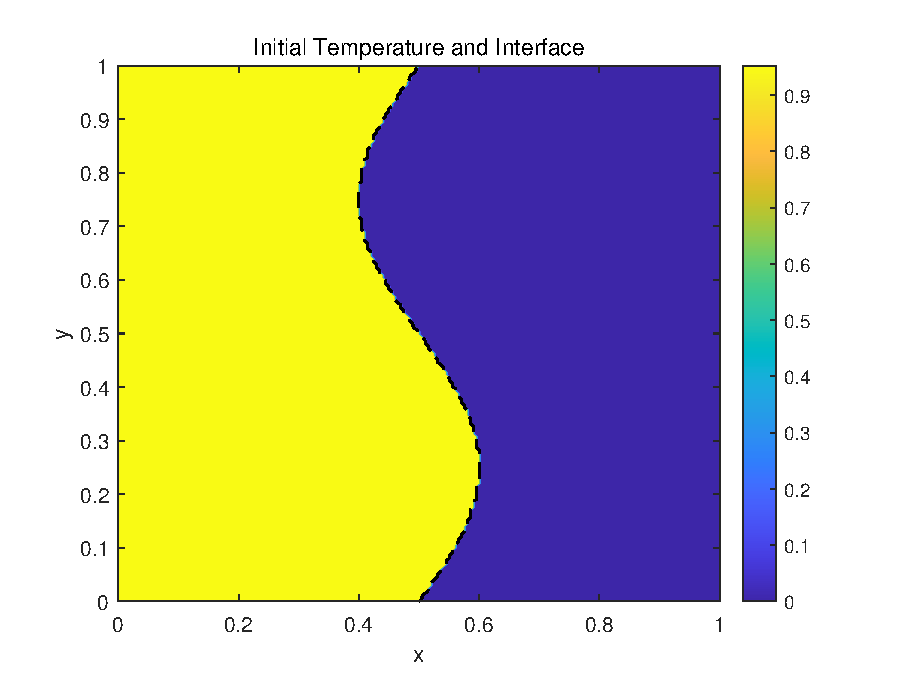
\includegraphics[width=\textwidth]{./figures/figure_16.eps}
    \label{fig:15a}
  \end{subfigure}
  \begin{subfigure}[b]{0.47\textwidth}
    \centering
    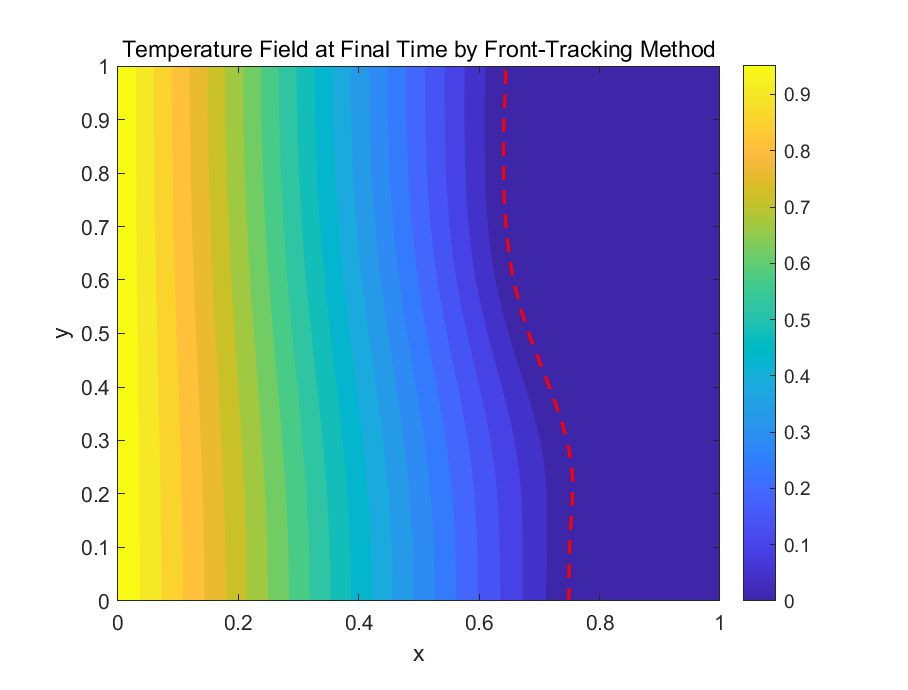
\includegraphics[width=\textwidth]{./figures/figure_17.eps}
    \label{fig:15b}
  \end{subfigure}
  \caption{The result of Front Tracking Method with grid number 200 at $t=0.1$}
  \label{fig:15}
\end{figure}

By comparison, we can see the result of front tracking method is very similar to the result of Enthalpy Method. Finally, I plot a simulation with a more complex initial condition which is a circle with radius $r = 0.4$ and center at $(0.5,0.5)$ as figure \ref{fig:18} which shows the temperature profile and the final interface position at $t=0.05$. By the experiment with Front Tracking Method, we can see the biggest advantage of this method is that it can handle the high dimensional case easily and easy to implement since it follows directly from the finite difference scheme, all the things we need to do is to track the interface position and update the temperature. The disadvantage is that it has to explicitly handle the interface position, which will potentially lead to numerical errors especially for the complex geometries. 
\begin{figure*}[h!]
  \centering 
  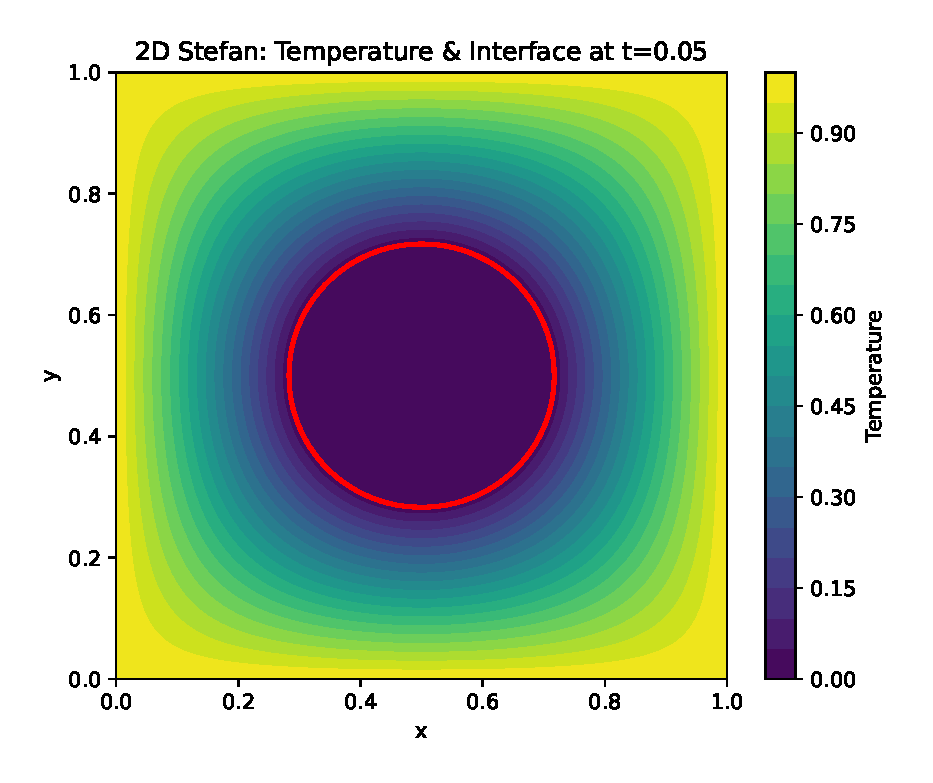
\includegraphics[width=0.5\textwidth]{./figures/figure_18.eps}
  \caption{The result of Front Tracking Method with initial interface as a circle at $t=0.05$}
  \label{fig:18}
\end{figure*}

\subsection*{Level Set Method}
For level set method, all the steps follow from the one dimensional case. The only thing need to be paid attention is for two dimensional case
\begin{equation*}
  \phi_t = \nabla T \cdot \nabla \phi, \quad \forall x \in \Gamma(t).
\end{equation*}
The re-initialization is same as the one dimensional case. And we also perform a test with the same initial condition as the front tracking method. The following figure shows the temperature profile and the final interface position at $t=0.1$.
The result indicate that the level set method is also valid for two dimensional Stefan problem. Also, by compare the error of Front Tracking Method and Level Set Method, we can see the level set method is more accurate than the front tracking method for two dimensional case. 
\begin{lstlisting}[style=Matlab-editor]
  With grid number 200, the error of interface position at final time is 8.035311e-04
\end{lstlisting}
\begin{figure*}
  \centering
  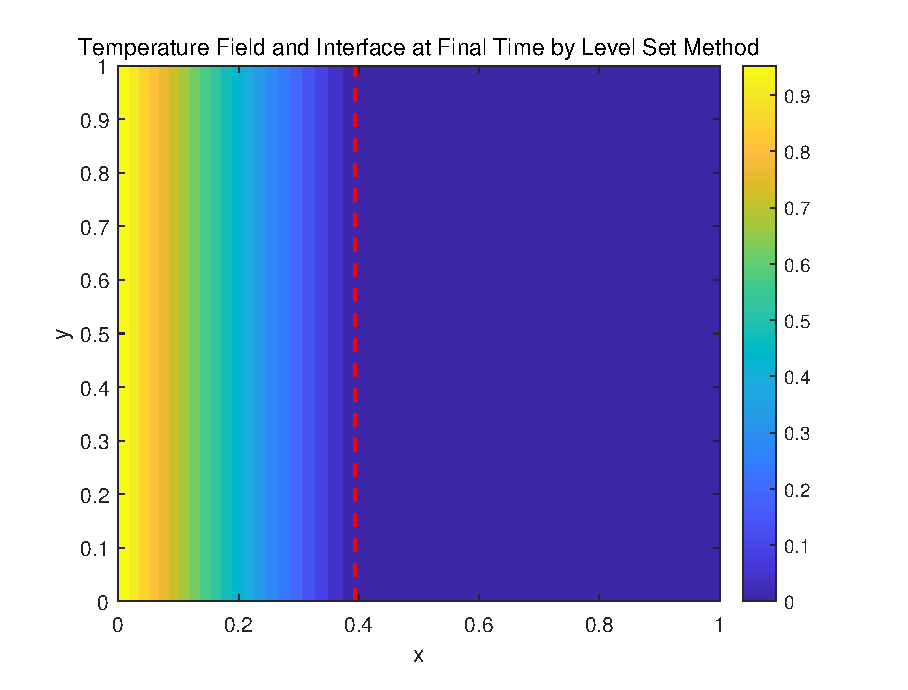
\includegraphics[width=0.55\textwidth]{./figures/figure_19.eps}
  \caption{The temperature profile and final interface position at $t=0.1$}
  \label{fig:19}
\end{figure*}
\begin{figure*}
  \centering
  \begin{subfigure}[b]{0.47\textwidth}
    \centering
    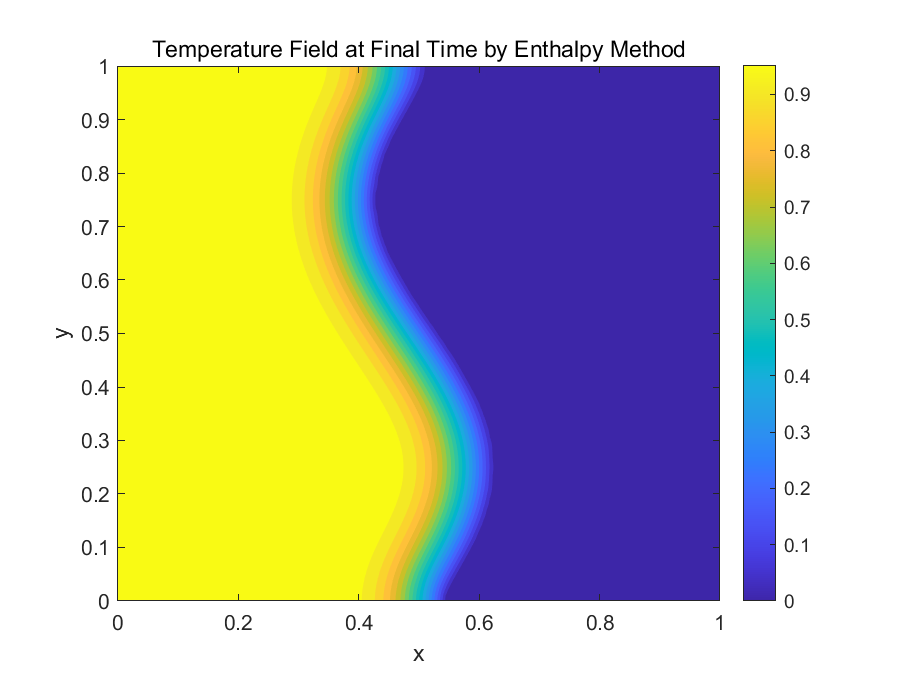
\includegraphics[width=\textwidth]{./figures/figure_20.eps}
    \label{fig:20a}
  \end{subfigure}
  \begin{subfigure}[b]{0.47\textwidth}
    \centering
    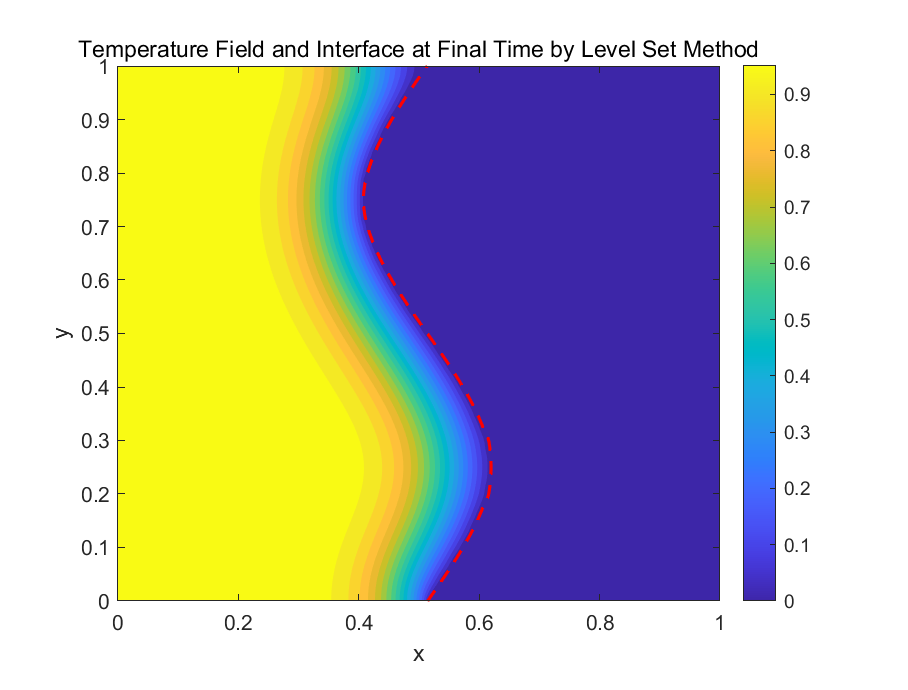
\includegraphics[width=\textwidth]{./figures/figure_21.eps}
    \label{fig:20b}
  \end{subfigure}
  \caption{The result with validation simulated by Enthalpy Method.}
  \label{fig:20}
\end{figure*}
\begin{figure*}[h!]
  \centering
  \begin{subfigure}[b]{0.47\textwidth}
    \centering
    \includegraphics[width=\textwidth]{./figures/output.png}
    \label{fig:22a}
  \end{subfigure}
  \begin{subfigure}[b]{0.47\textwidth}
    \centering
    \includegraphics[width=\textwidth]{./figures/output1.png}
    \label{fig:22b}
  \end{subfigure}
  \caption{Temperature profile and the level set function}
  \label{fig:22}
\end{figure*}
The I also check the result with the Enthalpy Method. Due to the cost of the Level Set Method, I only iterate 800 time steps, for both methods. From \ref{fig:20}, we can find both two methods yield the similar results. Finally, I plot the temperature profile and the level set function in figure \ref{fig:22}. The main advantage of the level set method is that it can handle the complex geometries easily since it is based on the implicit representation of the interface by the level set function. But the re-initialization process will be a little bit complex and time consuming, because it doesn't have an explicit solution, thus we need to apply method such as Runge-Kutta method to solve.

\section{Conclusion}
This project simulated the one and two dimensional Stefan problem using front tracking method and level set method. The results show that both methods are valid for the Stefan problem with the basic finite difference scheme for heat equation. Both methods yield about first order convergence for the interface position and temperature. The difficulty of the convergence order is due to the first order update equation for the interface position. To achieve higher order convergence for free boundary problem, simplely using the higher order finite difference scheme such as Crank-Nicholson method is not enough, we need to use the higher order method for the interface position.
\end{document}